\chapter{Hardware Detail Design}
\label{chap:5}

This chapter gives a detailed discussion on the hardware design and
configuration of this system. This includes the relay switching circuit, the
motor and coil design and the NFC chip configuration.

See Appendix \ref{add:d} for a schematic layout of the hardware and their
connections.

\section{Relay Switch Circuit}
\label{sec:detail-switch}

As explained in Section \ref{sec:relay-switch} in page \pageref{sec:relay-switch}, a relay
switch (the Mantech NT72C 12V DC relay [\cite{manual:relay-specs}]), in conjunction with a 2N2222
Bipolar Junction Transistor (BJT) [\cite{maunual:transistor-datasheet}], is used
by the Raspberry Pi to switch the motor on and off. See Figure
\ref{fig:relay-switch} for the circuit diagram.

\begin{figure}
\centering
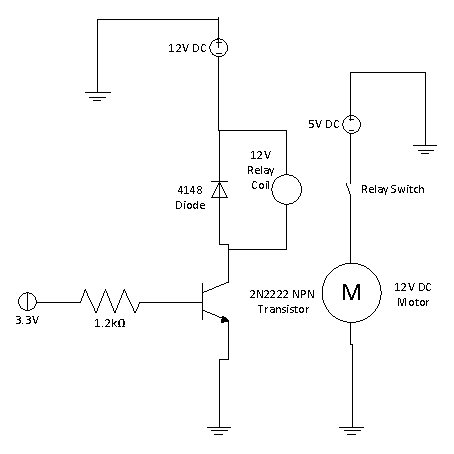
\includegraphics[clip = true, trim = 0 640 0 70, scale=1]{relay_switch}
\caption{12 V relay transistor switch.}
\label{fig:relay-switch}
\end{figure}

\begin{minipage}{\textwidth}

The variables used here are defined as follows:
\\\\
P$_r$\dotfill Relay coil power dissipation\\
V$_r$\dotfill Voltage across the relay\\
$\beta$\dotfill BJT current amplification\\
V$_p$\dotfill Voltage supply from a Raspberry Pi's GPIO pin\\
I$_p$\dotfill Current supply from a Raspberry Pi's GPIO pin\\
I$_b$\dotfill The BJT's base current\\
R$_b$\dotfill The BJT's base resistor\\

\end{minipage}

The relevant  parameters for these components are [\cite{manual:relay-specs},
\cite{maunual:transistor-datasheet}]:

\[ \mathrm{\ P_{r}} = 0.36\mathrm{\ W}\]
\[ \mathrm{\ V_{r}} = 12\mathrm{\ V}\]
\[ \mathrm{\ \beta} \approx 10\]
\[ \mathrm{\ V_{p}} = 3.3\mathrm{\ V}\]

From the relay's power dissipation and voltage, its current draw is found by

\[
\mathrm{\ I_{r}} = \frac{\mathrm{\ P_{r}}}{\mathrm{\ V_{r}}}
\]

which gives a current draw of

\[
\mathrm{\ I_{r}} = 0.03\mathrm{\ A}
\]

Taking the BJT's current amplification as roughly 10, as recommended by the
BJT's datasheet [\cite{maunual:transistor-datasheet}], the current draw from the
Pi to the base of the BJT is given by

\[
\mathrm{\ I_{b}} = \frac{\mathrm{\ I_{r}}}{\beta} = \frac{\mathrm{\
I_{c}}}{\beta}
\]

This gives a current draw of

\[
\mathrm{\ I_{b}} = 0.003\mathrm{\ A} = 3\mathrm{\ mA}
\]

The maximum current draw from the GPIO pins is 16 mA
[\cite{website:gpio-specs}], though this is not recommended as the Pi does not
have any current limiting or over-current protection.
Therefore, a current draw of 3 mA is completely safe.

To limit the current draw from the Pi, a base resistor must be added between the Pi's GPIO pin
and the BJT's base. With a current draw of 3 mA and a voltage of 3.3 V, the
resistor size is found by Ohm's law as follows

\[
\mathrm{\ R_{b}} = \frac{\mathrm{\ V_{p}}}{\mathrm{\ I_{p}}}
\]

which gives

\[
\mathrm{\ R_{b}} = 1.1\mathrm{\ k\Omega}
\]

To prevent voltage spikes from the Pi's GPIO's from supplying to much current, a
further 10\% was added to the resistor size. This gives a resistor size of

\[\mathrm{\ R_{b}} = 1.2\mathrm{\ k\Omega}\]

which draws a current of 

\[\mathrm{\ I_{b}} = 2.75\mathrm{\ mA} \]

which is still enough to activate the relay's coil and turn the motor on. 

\section{NFC Chip}

The Near Field Communication (NFC) chip used, is the Adafruit NFC shield for an
Arduino Uno microcontroller [\cite{website:adafruit-nfc}]. See Section
\ref{sec:nfc-controller} on page \pageref{sec:nfc-controller} for more details
on the controller.

The shield was designed and built to be used by an Arduino Uno microcontroller.
Therefore, some modification to the chip's connections had to be made before it
would be able to communicate with the Pi.

By default, the chip was made to communicate with an Arduino with the Inter
Integrated Circuit (i$^2$c) communication protocol. However, the component
manufacturers have added connection pads to the chip that, when soldered, allows
the chip to communicate via Serial Peripheral Interface (SPI) or Transistor
Transistor Login (TTL). 

The libnfc library is currently only configured to allow communication via an
Universal Asynchronous Receiver Transmitter (UART). Therefore, the chip was
modified to communicate via its TTL interface, which is compatible with the Pi's
UART interface.

To do this, the `SEL1' pads are shorted (see Figure
\ref{fig:nfc-chip-solder}). With this done, the chip can serially communicate
with the Raspberry Pi's UART interface.

\begin{figure}
 \centering 
 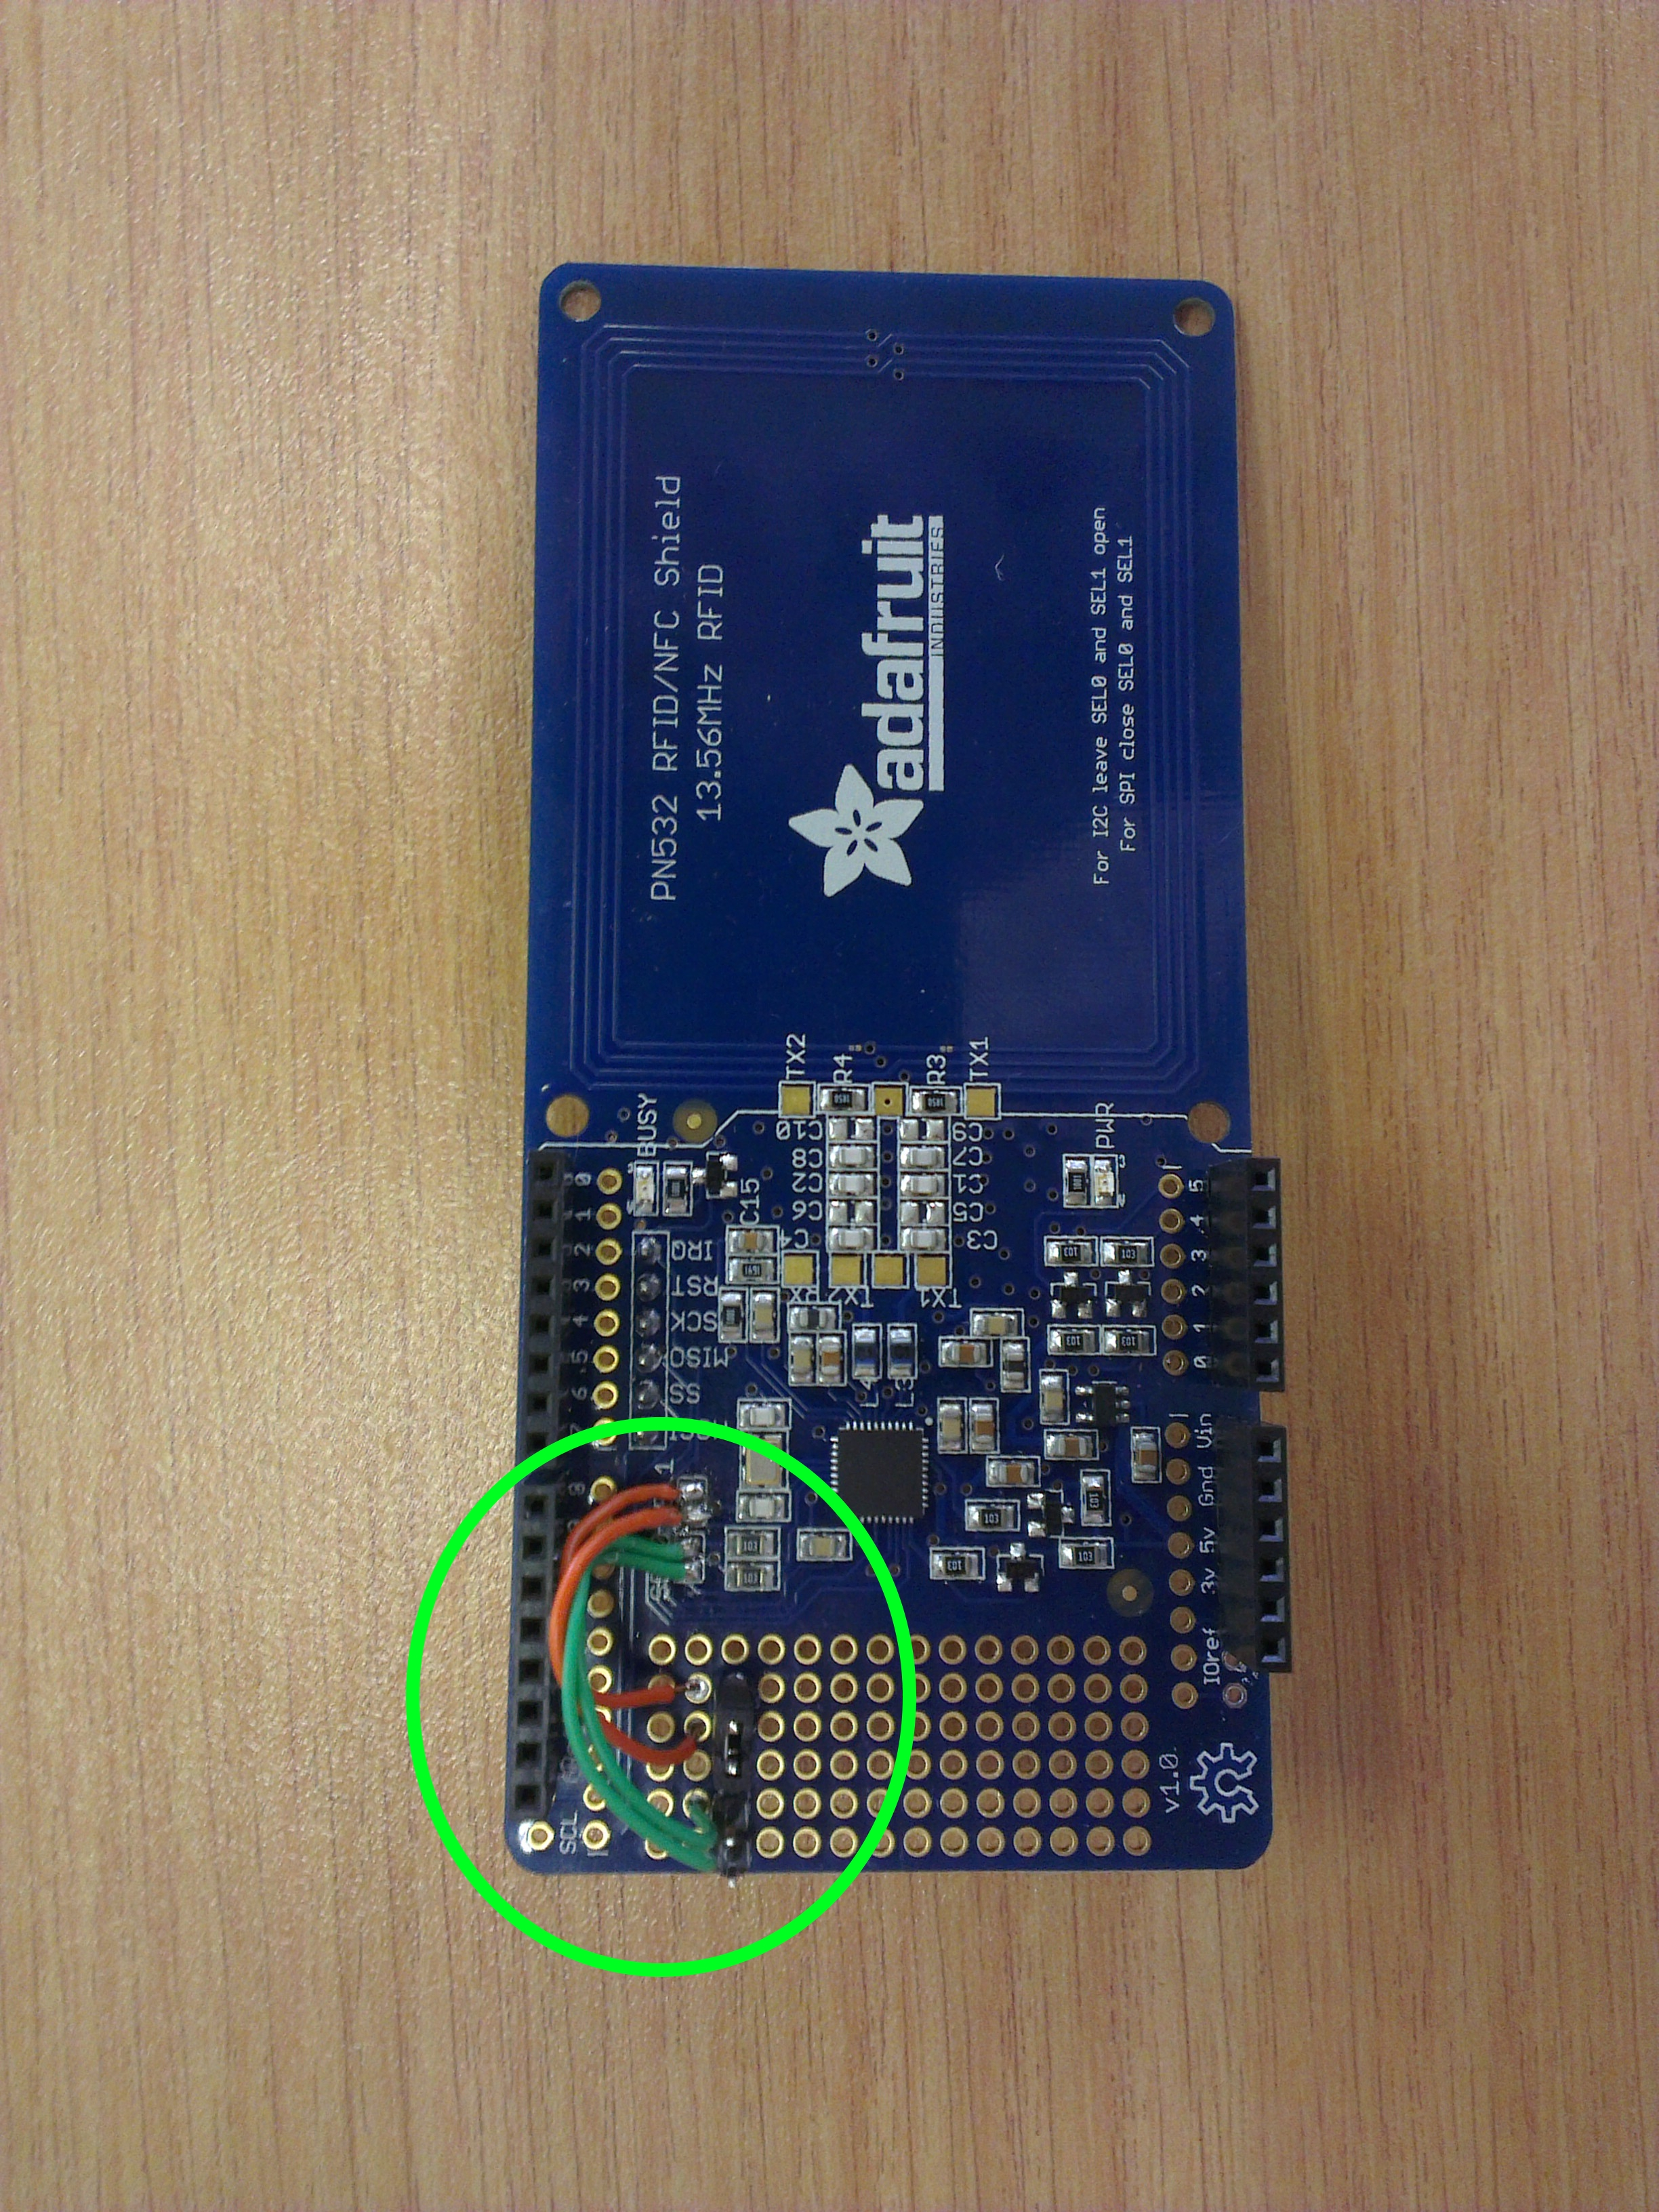
\includegraphics[clip=true, trim = 0 250 0 290,
 scale=0.7]{soldeer_pic}
 \caption{The location of the SEL1 pads (highlighted in green).}
 \label{fig:nfc-chip-solder}
\end{figure}

The connections between the Pi and the NFC controller are as follows: 

\begin{table}
\centering
 \caption{Connections between the Raspberry Pi and the NFC Controller chip.}
 \begin{tabular}{|l|l|l|}
  \hline
  \textbf{NCF Controller Pin} & \textbf{Raspberry Pi Pin}\\\hline\hline
  5V pin & 5V (pin 4) \\\hline
  Ground pin & Ground pin (pin 6) \\\hline
  SS & UART0 TXD (pin 8) \\\hline
  MOSI & UART0 RXD (pin 10) \\\hline
 \end{tabular}
\end{table}

\section{libnfc Setup on the Raspberry Pi}

Before libnfc could be built and configured, the communication between the NFC
controller and the Pi needed to be finalised. To do this, the Pi's UART needed
to be freed up. By default, the Raspberry Pi uses its UART to serially write out
its booting information. Therefore, to allow the Raspberry Pi to communicate
with the NFC controller via its UART0 interface, it was necessary to modify
some of its configuration files. To do this, the Adafruit tutorial was followed
[\cite{website:adafruit-tutorial}].

The file `/boot/cmdline.txt' and `/etc/inittab' had to be edited to
contain the following lines of code:

\textbf{cmdline.txt}
\begin{verbatim}
dwc_otg.lpm_enable=0 console=tty1
\end{verbatim}

\textbf{inittab}
\begin{verbatim}
#Spawn a getty on Raspberry Pi serial line
#T0:23:respawn:/sbin/getty -L ttyAMA0 115200 vt100
\end{verbatim}

After this has been done, the libnfc package could be configured and installed 
to work with the Pi's UART interface.

Thereafter, the Pi was ready to receive NFC messages from the NFC shield.

\section{Vending Machine Unit}

A small vending machine unit was constructed for demonstration purposes. It is
designed to house all the vending machine components, i.e. the two DC motors,
the two coils, the Raspberry Pi central controller, the NFC shield and the
webcam.

Four 10 mm vent holes were added at the sides to improve air circulation
and to provide external wire access, while a larger 60 mm vent hole was also
added to allow for an external 60 mm desktop computer fan to be added at a
later stage.

The unit is made from 1.6 mm thick mild steel and the components were cut and
bent by Fabrinox, Paarl and welded together by the Electrical and Electronic
Engineering Department of Stellenbosch University's workshop.

See Figure \ref{fig:vm-actual} for a picture of the complete vending machine
unit with the two DC motor inserted. See Appendix \ref{app:vm-tekeninge} for
detailed design drawings of the vending machine unit.

\begin{figure}
 \centering 
 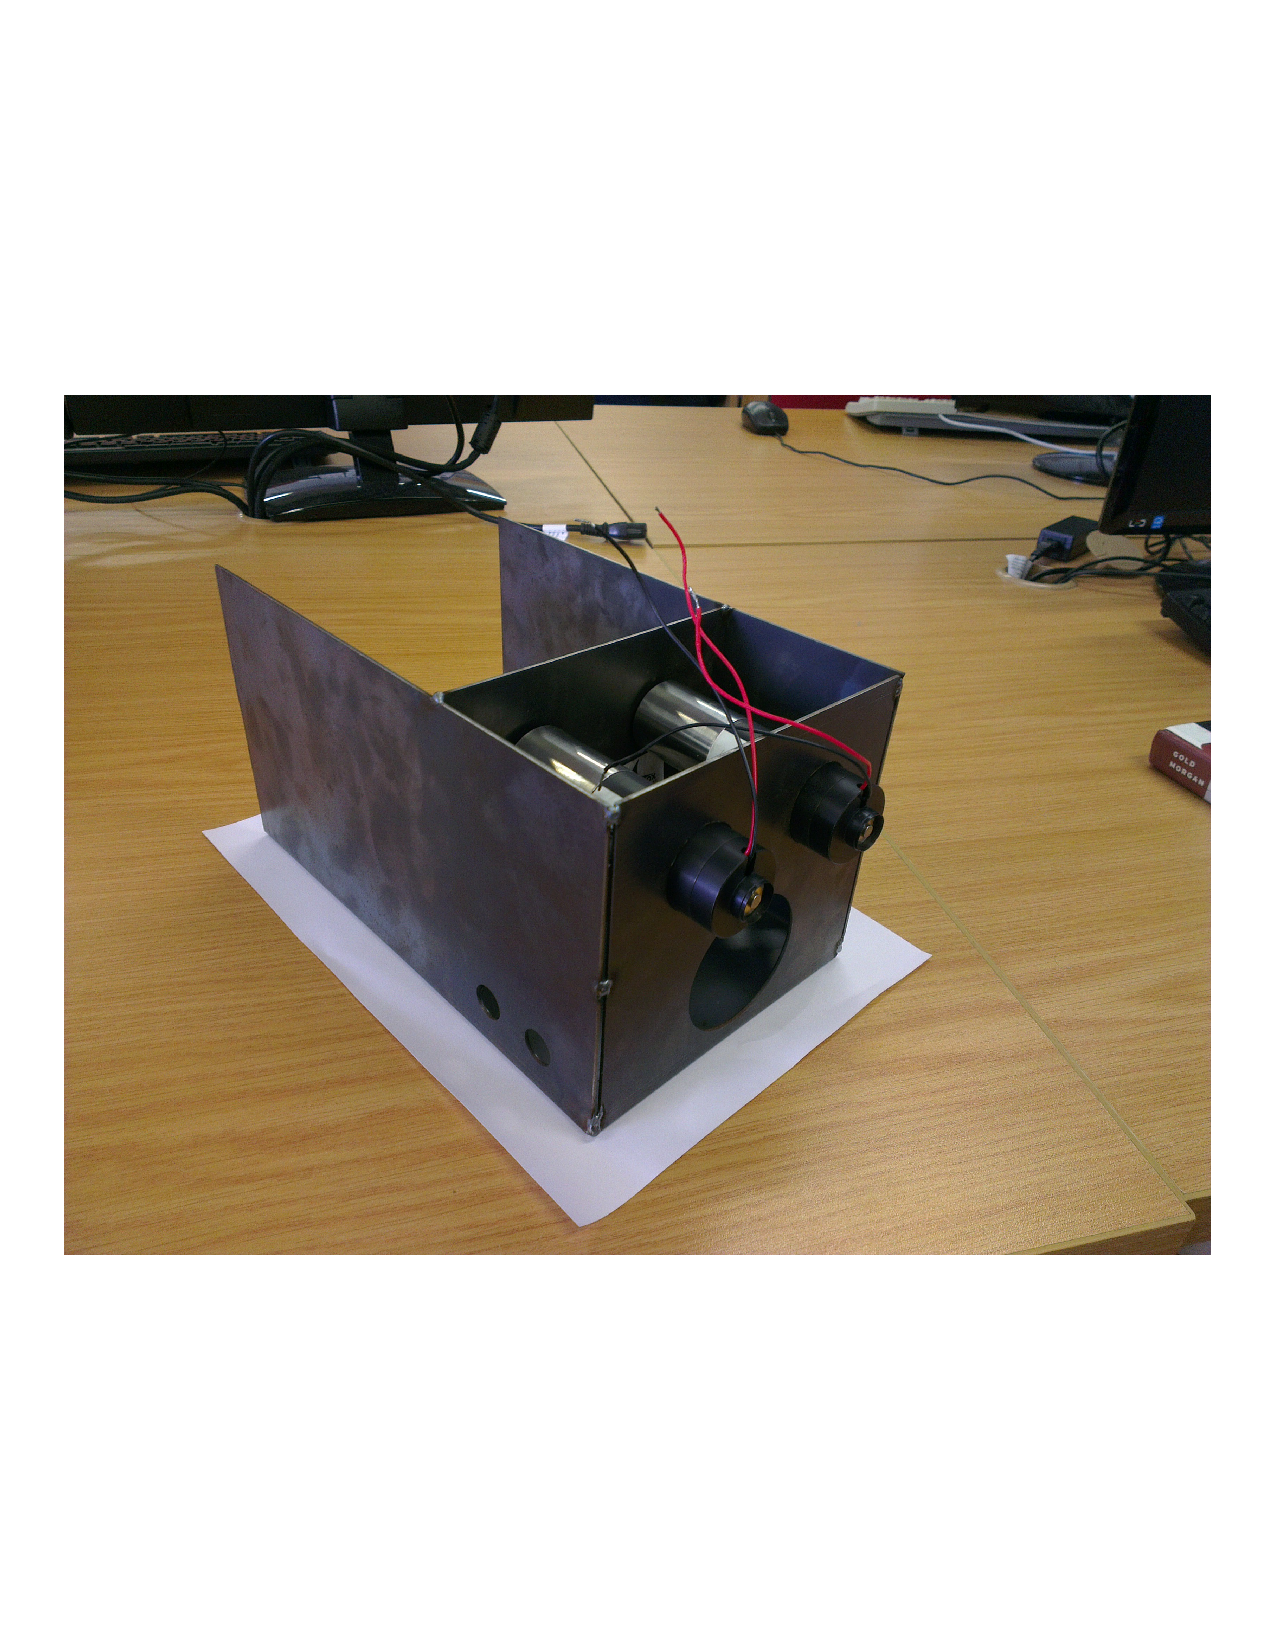
\includegraphics[clip=true, trim = 80 180 150 200,
 scale=0.7]{complete_vm}
 \caption{The complete vending machine unit.}
 \label{fig:vm-actual}
\end{figure}

\section{Webcam}

As discussed in Section \ref{sec:webcam}, a Sony PS2 Eye Toy  webcam was
attached to the Raspberry Pi. This allows the vending machine to scan a live
video feed for a QR Code. It is already compatible with the Raspberry Pi and
therefore requires minimal configuration to begin working.

It is important to note that a Raspbian version from early 2013 was used on the
Raspberry Pi. It was found that the latest Raspbian distributions have an
unknown bug in its Video4Linux (v4l) video drivers which causes the EyeToy to
work incorrectly. 

Furthermore, the camera needs to be plugged into a Universal Serial Bus (USB)
port on the Pi itself and not into an external USB hub. This is done in order to
prevent hardware timing issues that are introduced to the system when a USB hub is used.

\section{Motor and Coil}

The vending machine dispenses products by activating a motor that turns a coil
loaded with a product. This turning motion causes a product to move along the
coil in an Archimedean screw-like manner until it falls off at the end of the
coil. 

In the demonstration vending machine, two coils are used. The coils are made
from 2.5 mm thick galvanised iron wire. The coil diameter is 50 mm and has a
longitudinal pitch of 20 mm. 

It is important for the motor to only be activated for one turn of the coil to
ensure that only one product is dispensed per completed transaction. This is
currently being done by only activating a motor for a set amount of time.To
determine this time, it was first required that the speed of the motor be
determined for a given supply voltage.

The motors that are used are 12 V DC motors made by Faulhaber
[\cite{manual:dc-motors}] coupled with a 14:1 speed gearbox
[\cite{manual:gearbox}].

%\begin{minipage}{\textwidth}
The variables used in the following equations are defined as follows:\\\\
V$_o$\dotfill Motor supply voltage\\
I\dotfill Current supply to motor\\
R\dotfill DC Motor terminal resistance\\
V$_e$\dotfill Reverse Electromotive Force (EMF) voltage\\
$\omega$\dotfill Motor speed\\
k$_e$\dotfill Back-EMF constant\\
%\end{minipage}

The following equation gives the relationship between a DC motor's supply
voltage and its reverse Electromotive Force (EMF).

\[ \mathrm{V}_o = \mathrm{IR} + \mathrm{V}_e\]

The reverse EMF is proportional to the rotational speed of the motor. Therefore,
the V$_e$ term can be taken as

\[ \mathrm{V}_e = \omega\mathrm{k}_e\]

which gives the following equation

\begin{equation}
 \label{eq:motor}
 \mathrm{V}_o = \mathrm{IR} + \omega\mathrm{k}_e
\end{equation}

The IR term is taken as constant as the loading on the motor stays the same.
From the motor's datasheets and usage tests, the I, R and k$_e$ terms were
determined to have the following values:

\[\mathrm{I} = 0.35\mathrm{\ A}\]
\[\mathrm{R} = 0.41\mathrm{\ \Omega}\]
\[ \mathrm{k}_e = 2 \mathrm{\ mV/rpm}\]

Using these values and setting the input voltage as 3.3 V in equation
\ref{eq:motor}, the motor's speed was determined to be 113 RPM. Therefore, to
complete a single revolution, the motor may only be activated for 0.53 seconds. 

This is not the most effective method, however, because the errors in the system
accumulate over time. In time, these errors may lead incorrect product
dispensing. 

To improve this, a proximity sensor may be added onto the coil and onto the
vending machine wall. This sensor can be connected to and be controlled by the
Raspberry Pi and would be activated every time the coil completes one
revolution. When the sensor is triggered, the Pi will then know that exactly
one revolution has been completed and stop the motor. This will stop any errors
from accumulating over time and make the vending machine more reliable. 
